\documentclass[12pt,a4paper]{article}

\usepackage[utf8]{inputenc}
\usepackage[T2A]{fontenc}
\usepackage[russian]{babel}
\usepackage{amsmath,amssymb}
\usepackage{graphicx}
\usepackage{booktabs}
\usepackage{multirow}
\usepackage{geometry}
\usepackage{float}
\usepackage{eso-pic}
\graphicspath{{./}}

\geometry{top=2cm,bottom=2cm,left=2.5cm,right=1.5cm}

\title{\textbf{Лабораторная работа 1.1.4}\\
Изучение статистических закономерностей на примере измерения фона космического излучения}

\author{
    Студент \underline{Шеховцов Василий Максимович}\\
    Группа \underline{Б03-601}\\
    Преподаватель \underline{Ивлев Д.А.}
}

\date{
Московский Физико-технический институт\\
(национальный исследовательский университет)\\
22 сентября 2026 г.
}

\begin{document}

\AddToShipoutPictureFG*{
    \AtPageUpperLeft{
        \hspace{1.5cm}
        \raisebox{-1cm}{
            \makebox[0pt][l]{Шеховцов В.М.}
        }
    }
}

\maketitle

\section*{Цель работы}

На примере статистики регистрации фоновых космических частиц изучить статистические закономерности однородного
во времени случайного процесса; проверить возможность описания исследуемого процесса статистическими законами Пуассона и Гаусса;
измерить среднее число регистрируемых космических лучей в секунду и определить погрешность результата.

\section*{Оборудование}

\begin{itemize}
    \item Счётчик Гейгера--Мюллера (СТС-6);
    \item блок питания;
    \item компьютер с интерфейсом связи со счётчиком и расчётная программа.
\end{itemize}

\section*{1. Теоретические сведения}

Радиоактивным излучением называют потоки частиц (протонов, электронов и позитронов,
альфа-частиц, нейтронов и т.п.) или электромагнитных волн, способных вызывать ионизацию вещества.

Основными источниками радиации являются космические лучи и распад радиоактивных веществ.

Основную часть фона обычно составляет космическое излучение, которое исходно состоит из
протонов ($\approx 85\%$), альфа-частиц ($\approx 10\%$),
ядер более тяжёлых элементов ($<5\%$) и электронов и позитронов ($\approx 1\%$).

При взаимодействии этих лучей с атмосферой Земли рождается разнообразное множество нестабильных частиц
(мюоны, пи-мезоны и др.).

\subsection*{Устройство счётчика Гейгера--Мюллера}

Счётчик Гейгера--Мюллера представляет собой наполненный газом металлический цилиндр с двумя электродами. Одним из электродов (катодом) служит сам корпус, другим (анодом) — тонкая нить, натянутая вдоль оси цилиндра. Необходимое напряжение (400~В) подаётся на счётчик от блока питания.

\begin{figure}[H]
    \centering
    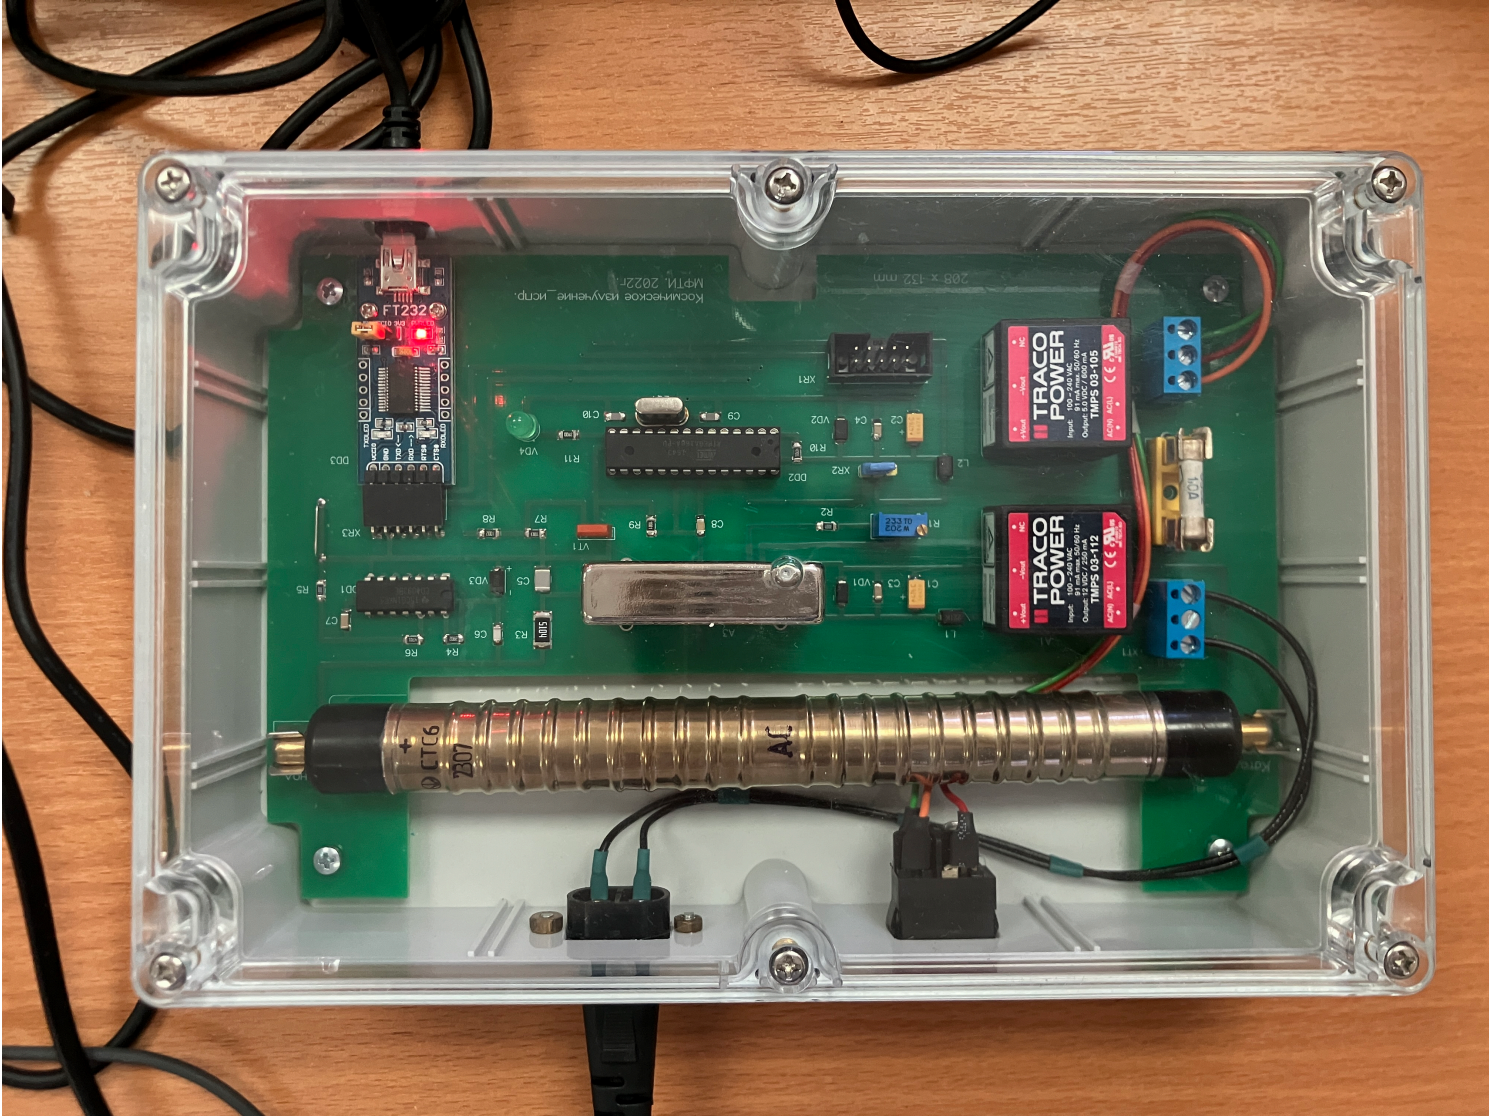
\includegraphics[width=0.8\textwidth]{geiger.png}
    \caption{Схема устройства счётчика Гейгера--Мюллера}
    \label{fig:geiger}
\end{figure}

Радиоактивное излучение ионизует молекулы газа, которым наполнен счётчик, а также выбивает электроны из его стенок. Образовавшиеся электроны, ускоряясь в сильном электрическом поле между электродами счётчика, соударяются с молекулами газа, выбивая из них новые вторичные электроны. В результате образуется лавина электронов, и через счётчик протекает кратковременный импульс тока. Этот импульс регистрируется электрической цепью установки, оцифровывается и через USB-интерфейс передаётся на компьютер.

\subsection*{Статистическая обработка данных: базовые сведения}

Результат любого физического измерения содержит погрешности. Частным случаем случайных погрешностей являются статистические погрешности, вызываемые случайными колебаниями (флуктуациями) самой измеряемой величины. К числу таких флуктуирующих величин относится и интенсивность космического излучения.

Пусть при некотором измерении за время $\tau$ зарегистрировано $n$ космических частиц. Из этого не следует, что в любые следующие $\tau$ секунд будет регистрироваться то же число частиц: в силу случайных причин можно получить любое другое значение, не слишком сильно отличающееся от $n$. Поэтому физический смысл имеет не результат отдельного измерения, а совокупность множества результатов и её усреднённые характеристики.

Выборочное среднее значение числа регистрируемых частиц:

\begin{equation}
    \langle n\rangle \equiv \frac{1}{N}\sum_{i=1}^{N} n_i.
    \label{eq:mean}
\end{equation}

Мера флуктуаций значений $n_i$ около среднего — среднеквадратичное (стандартное) отклонение, определяемое через выборочную дисперсию:

\begin{equation}
    \sigma_n^2 \equiv \frac{1}{N}\sum_{i=1}^{N}(n_i - \langle n\rangle)^2.
    \label{eq:variance}
\end{equation}

Погрешность среднего значения при независимых измерениях связана со стандартным отклонением отдельного измерения формулой

\begin{equation}
    \sigma_{\langle n\rangle} = \frac{\sigma_n}{\sqrt{N}}.
    \label{eq:mean_error}
\end{equation}

Истинное среднее значение $\bar n$ с высокой вероятностью лежит в интервале

\begin{equation}
    \bar n = \langle n\rangle \pm \sigma_{\langle n\rangle}.
    \label{eq:final_result}
\end{equation}

\subsection*{Распределение Пуассона}

Если случайные события (регистрация частиц) однородны во времени, а каждое последующее событие не зависит от предыдущих, такой процесс называется пуассоновским. Вероятность зарегистрировать $n$ частиц описывается распределением Пуассона:

\begin{equation}
    w_n = \frac{\bar n^{\,n}}{n!}\,e^{-\bar n},
    \label{eq:poisson}
\end{equation}

где $\bar n$ — единственный параметр распределения, совпадающий со средним числом частиц.

Наиболее характерное свойство распределения Пуассона — равенство среднеквадратичного отклонения корню из среднего значения:

\begin{equation}
    \sigma_n \approx \sqrt{\langle n\rangle}.
    \label{eq:poisson_property}
\end{equation}

При $\bar n \gtrsim 10$ распределение Пуассона приближается к нормальному распределению (распределению Гаусса), для которого известно, что отдельное измерение отличается от среднего не более чем на $\sigma$ с вероятностью 68{,}3\%, не более чем на $2\sigma$ — с вероятностью 95{,}4\%, и не более чем на $3\sigma$ — с вероятностью 99{,}7\%.

Относительная погрешность определения среднего значения интенсивности не зависит от выбора интервала группировки $\tau$ и убывает обратно пропорционально корню из полного числа зарегистрированных частиц $n_\Sigma = \langle n\rangle N$:

\begin{equation}
    \varepsilon_{\langle n\rangle} = \frac{1}{\sqrt{n_\Sigma}}.
    \label{eq:rel_error}
\end{equation}

\section*{2. Измерения и обработка данных}

Измерения проводились счётчиком Гейгера--Мюллера при напряжении 400~В в течение $t=4000$~с. Число зарегистрированных частиц записывалось компьютером с интервалом $\tau_0=1$~с, всего было получено 4000 отсчётов.

Для исследования статистических закономерностей исходная последовательность была разбита на группы с различным количеством последовательных измерений. Были рассмотрены четыре значения времени группировки:

\[
\tau=10,\ 20,\ 40,\ 80~\text{с}.
\]

При этом число независимых групп для каждого значения $\tau$ определялось выражением

\begin{equation}
    N=\frac{4000}{\tau}.
    \label{eq:N}
\end{equation}

Таким образом, для $\tau=10$~с получено $N=400$ измерений, для $\tau=20$~с --- $N=200$, для $\tau=40$~с --- $N=100$, а для $\tau=80$~с --- $N=50$.

Для каждой группы определялось суммарное число зарегистрированных частиц $n_i$. По полученной выборке рассчитывались среднее значение $\langle n\rangle$, среднеквадратичное отклонение $\sigma_n$, погрешность среднего $\sigma_{\langle n\rangle}$, интенсивность регистрации $j$ и её погрешность $\sigma_j$.

Среднее число зарегистрированных частиц, среднеквадратичное отклонение и погрешность среднего вычислялись по формулам~\eqref{eq:mean}, \eqref{eq:variance} и \eqref{eq:mean_error} соответственно. Использовалась выборочная дисперсия с множителем $1/N$; при $N\ge 50$ отличие от оценки с множителем $1/(N-1)$ пренебрежимо мало.

Интенсивность регистрации частиц определялась как

\begin{equation}
    j=\frac{\langle n\rangle}{\tau},
    \label{eq:intensity}
\end{equation}

а её погрешность:

\begin{equation}
    \sigma_j=\frac{\sigma_{\langle n\rangle}}{\tau}.
    \label{eq:intensity_error}
\end{equation}

Результаты расчётов представлены в таблице~\ref{tab:statistics}.

\begin{table}[H]
\centering
\caption{Статистические характеристики результатов измерений}
\label{tab:statistics}
\begin{tabular}{c|c|c|c|c|c|c}
\toprule
$\tau$, с & $N$ & $\langle n\rangle$ & $\sigma_n$
& $\sigma_{\langle n\rangle}$ & $j$, с$^{-1}$ & $\sigma_j$, с$^{-1}$ \\
\midrule
10 & 400 & 9.305 & 3.582 & 0.179 & 0.9305 & 0.0179 \\
20 & 200 & 18.61 & 5.270 & 0.373 & 0.9305 & 0.0186 \\
40 & 100 & 37.22 & 7.886 & 0.789 & 0.9305 & 0.0197 \\
80 & 50  & 74.44 & 12.764 & 1.805 & 0.9305 & 0.0226 \\
\bottomrule
\end{tabular}
\end{table}

Из таблицы видно, что среднее число зарегистрированных частиц $\langle n\rangle$ увеличивается пропорционально времени группировки $\tau$. При этом интенсивность регистрации для всех четырёх вариантов группировки имеет одинаковое значение:

\begin{equation}
    j=0.9305~\text{с}^{-1}.
\end{equation}

\subsection*{2.1. Проверка свойства распределения Пуассона}

Согласно распределению Пуассона, среднеквадратичное отклонение связано со средним числом зарегистрированных частиц соотношением

\begin{equation}
    \sigma_{n,\text{теор}}=\sqrt{\langle n\rangle}.
    \label{eq:sigma_theory}
\end{equation}

Для каждого значения $\tau$ была рассчитана теоретическая величина $\sqrt{\langle n\rangle}$ и сравнена с экспериментальным значением $\sigma_n$.

\begin{table}[H]
\centering
\caption{Сравнение экспериментального и теоретического отклонения}
\label{tab:poisson}
\begin{tabular}{c|c|c|c}
\toprule
$\tau$, с & $\sigma_n$ & $\sqrt{\langle n\rangle}$ &
$|\sigma_n-\sqrt{\langle n\rangle}|$ \\
\midrule
10 & 3.582 & 3.050 & 0.532 \\
20 & 5.270 & 4.314 & 0.956 \\
40 & 7.886 & 6.101 & 1.785 \\
80 & 12.764 & 8.628 & 4.136 \\
\bottomrule
\end{tabular}
\end{table}

Во всех случаях экспериментальное значение $\sigma_n$ оказывается несколько больше теоретического значения $\sqrt{\langle n\rangle}$. При этом с увеличением времени группировки $\tau$ среднее число зарегистрированных частиц и среднеквадратичное отклонение возрастают.

Полученные результаты в целом позволяют проверить характерную для распределения Пуассона зависимость между средним значением и величиной флуктуаций.

\subsection*{2.2. Проверка соответствия нормальному распределению}

Для проверки соответствия экспериментальных данных нормальному распределению была определена доля измерений, попавших в интервалы

\[
\langle n\rangle\pm\sigma_n,
\]

\[
\langle n\rangle\pm2\sigma_n,
\]

\[
\langle n\rangle\pm3\sigma_n.
\]

Для нормального распределения теоретические значения долей попаданий составляют приблизительно $68.3\%$, $95.4\%$ и $99.7\%$ соответственно.

Полученные экспериментальные значения представлены в таблице~\ref{tab:fractions}.

\begin{table}[H]
\centering
\caption{Доли измерений в интервалах вокруг среднего значения}
\label{tab:fractions}
\begin{tabular}{c|c|c|c}
\toprule
$\tau$, с & $\pm\sigma_n$ & $\pm2\sigma_n$ & $\pm3\sigma_n$ \\
\midrule
10 & 68.5\% & 93.0\% & 100.0\% \\
20 & 67.5\% & 95.0\% & 100.0\% \\
40 & 67.0\% & 95.0\% & 100.0\% \\
80 & 68.0\% & 94.0\% & 100.0\% \\
\bottomrule
\end{tabular}
\end{table}

Экспериментальные значения для интервала $\pm\sigma_n$ находятся в диапазоне от $67.0\%$ до $68.5\%$ и близки к теоретическому значению $68.3\%$.

Для интервала $\pm2\sigma_n$ получены значения от $93.0\%$ до $95.0\%$, что также близко к теоретическому значению $95.4\%$.

Во всех случаях в интервал $\pm3\sigma_n$ попало $100\%$ измерений. Теоретически за пределами этого интервала ожидается около $0.3\%$ измерений, то есть примерно одно измерение при $N=400$ и менее одного при остальных $N$. Поэтому отсутствие выходов за $3\sigma_n$ статистически совместимо с теоретическим значением $99.7\%$.

Таким образом, экспериментальные значения долей попаданий в интервалы $\pm\sigma_n$, $\pm2\sigma_n$ и $\pm3\sigma_n$ хорошо согласуются с ожидаемыми для нормального распределения значениями. Поскольку интервалы построены по выборочному $\sigma_n$, эта проверка касается формы распределения, а не соотношения $\sigma_n=\sqrt{\langle n\rangle}$. Форма распределения числа зарегистрированных частиц близка к нормальной, что согласуется с гауссовым приближением распределения Пуассона при $\langle n\rangle\gtrsim10$.

\subsection*{2.3. Распределение частот}

Для каждого значения времени группировки $\tau$ были построены гистограммы распределения относительных частот $w_n$ числа зарегистрированных частиц.

По оси абсцисс откладывалось число зарегистрированных частиц $n$, а по оси ординат --- относительная частота

\begin{equation}
    w_n=\frac{N_n}{N},
    \label{eq:frequency}
\end{equation}

где $N_n$ --- количество измерений, в которых было зарегистрировано $n$ частиц, а $N$ --- общее количество измерений для выбранного значения $\tau$.

На рисунке~\ref{fig:all_histograms} представлены гистограммы распределения числа зарегистрированных частиц для всех четырёх значений времени группировки $\tau$, наложенные друг на друга. График позволяет наглядно сравнить изменение распределения при увеличении времени группировки.

\begin{figure}[H]
    \centering
    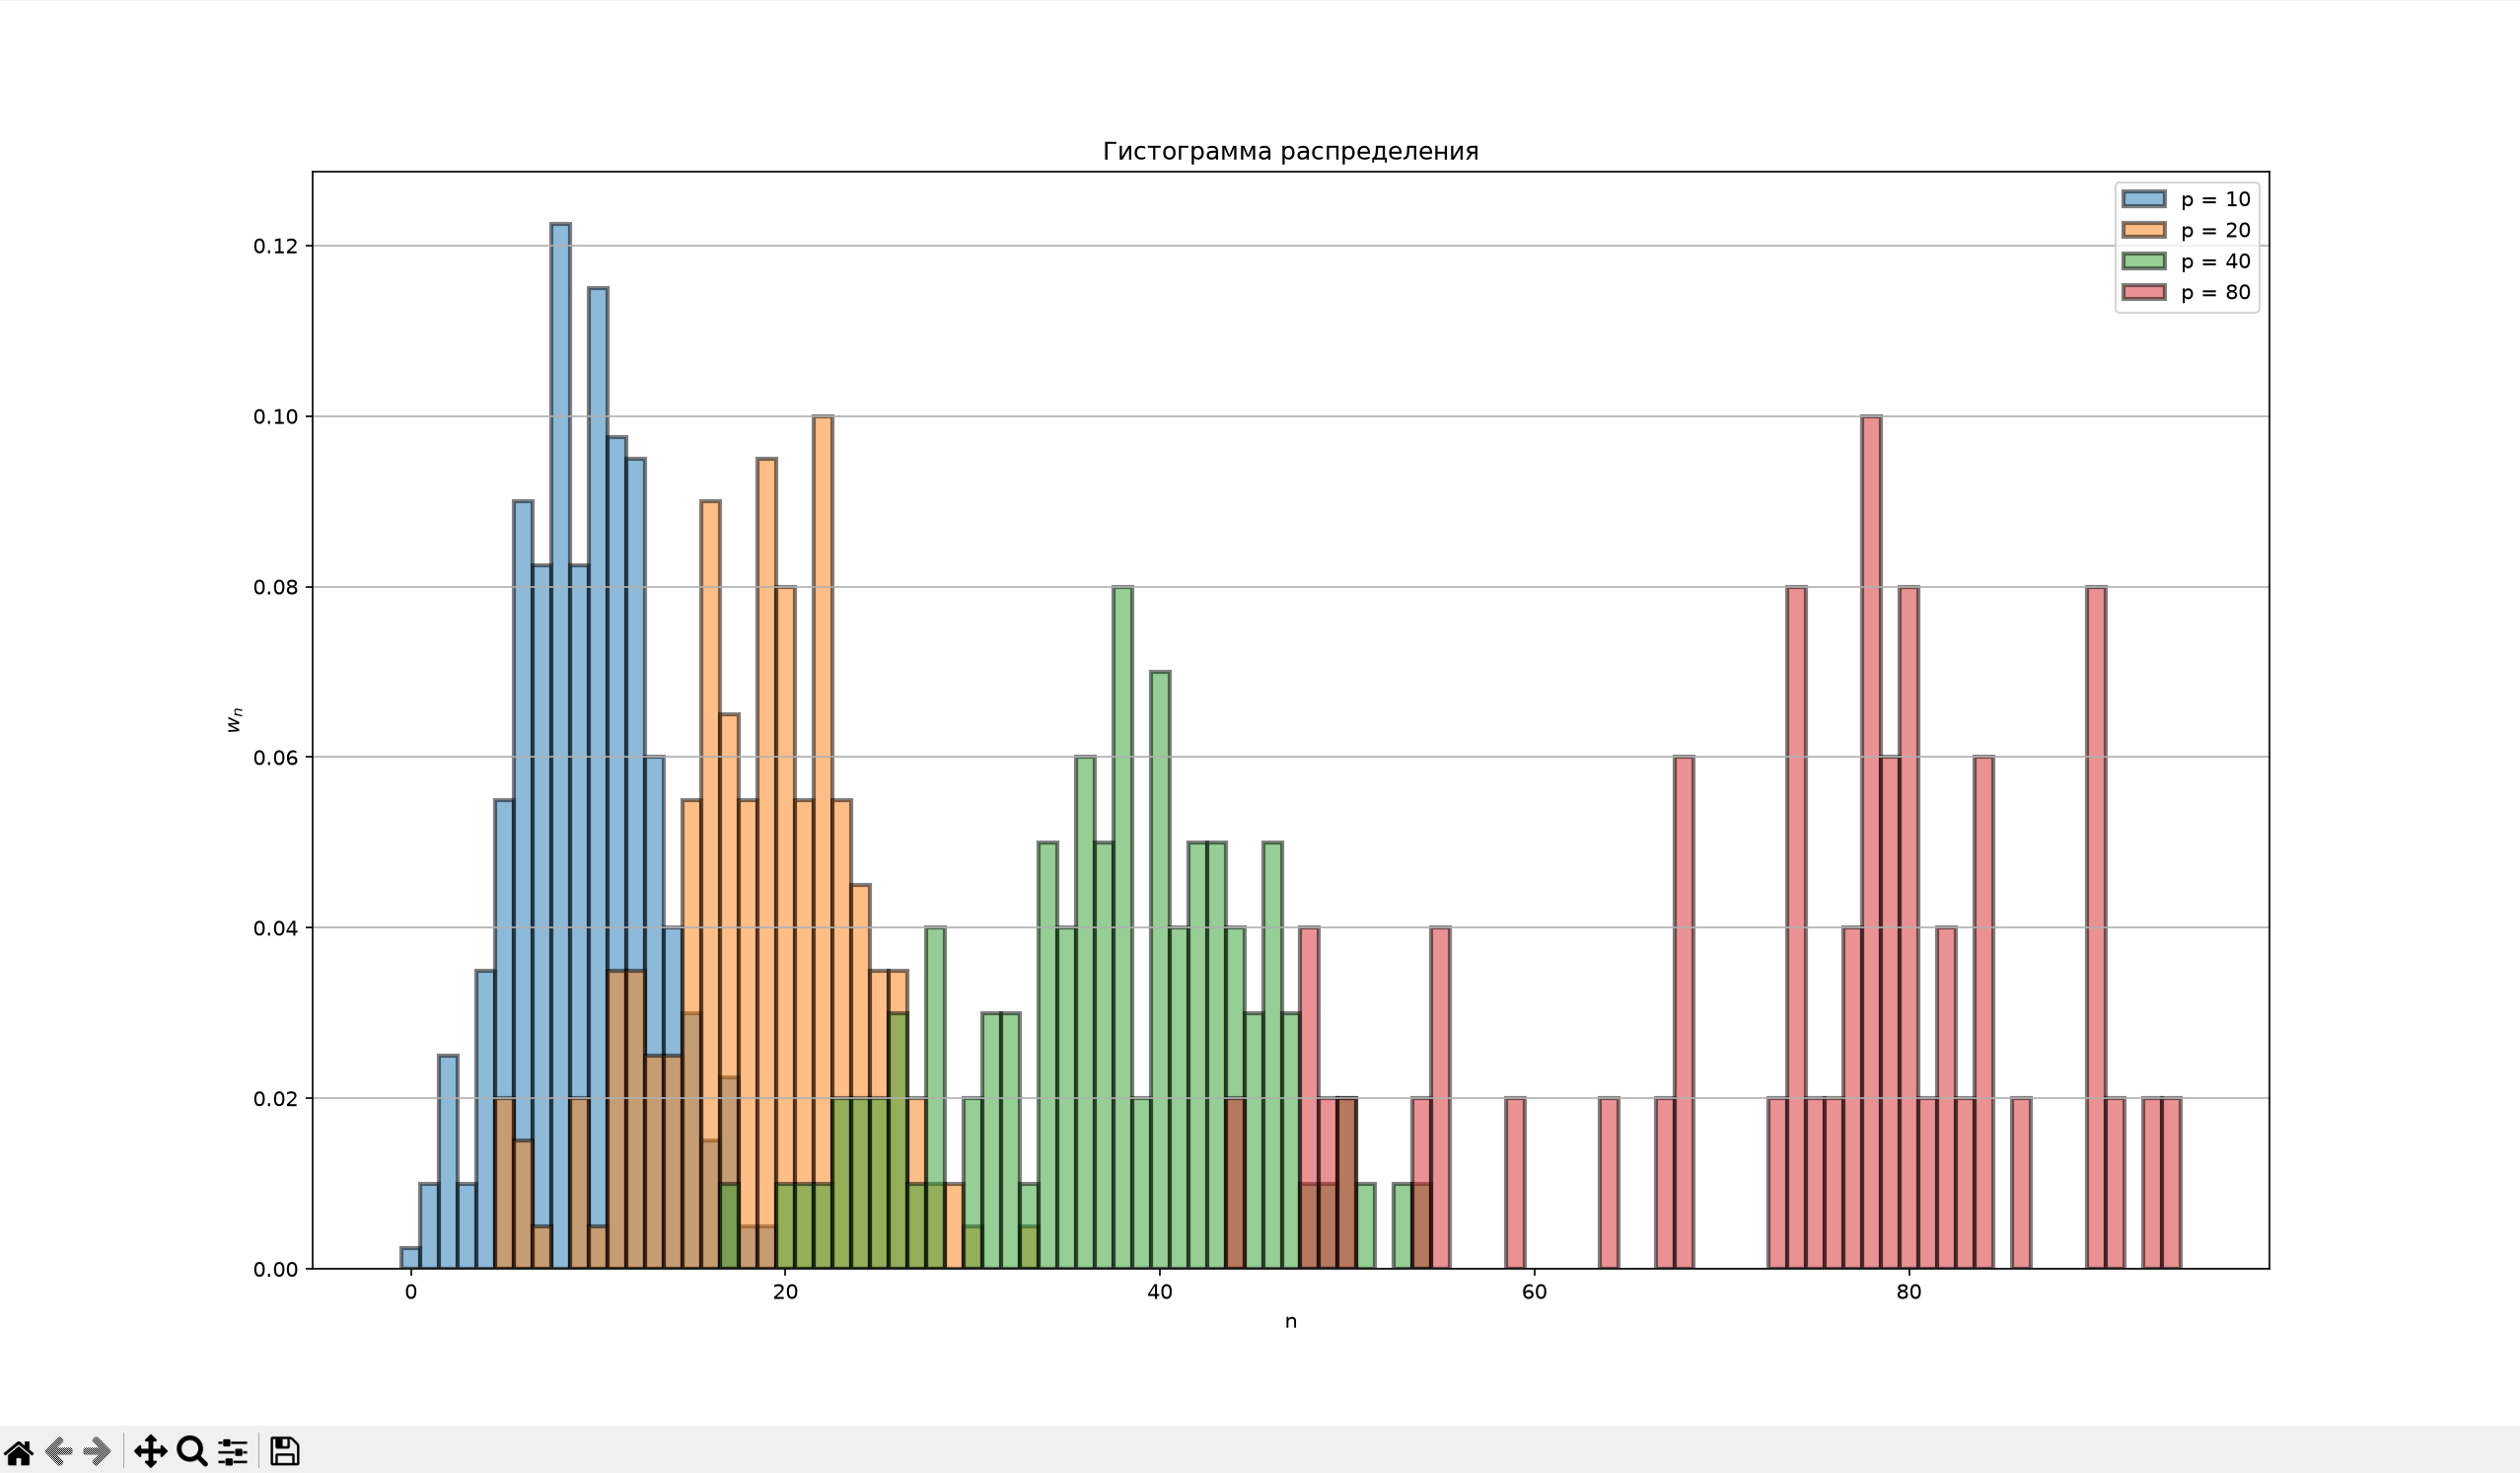
\includegraphics[width=0.85\textwidth]{15point.png}
    \caption{Гистограммы распределения числа зарегистрированных частиц для $\tau=10$, $20$, $40$ и $80$~с}
    \label{fig:all_histograms}
\end{figure}

Для $\tau=20$~с дополнительно было проведено сравнение экспериментальной гистограммы с распределением Пуассона

\begin{equation}
    w_n=\frac{\langle n\rangle^n}{n!}e^{-\langle n\rangle}
\end{equation}

и нормальным распределением

\begin{equation}
    w(n)=
    \frac{1}{\sigma_n\sqrt{2\pi}}
    \exp\left[
    -\frac{(n-\langle n\rangle)^2}{2\sigma_n^2}
    \right].
\end{equation}

Для $\tau=20$~с параметры распределений имеют значения

\[
\langle n\rangle=18.61,
\qquad
\sigma_n=5.270.
\]

При таком среднем значении распределение Пуассона уже достаточно близко к нормальному, поэтому обе теоретические кривые можно использовать для качественного сравнения с экспериментальной гистограммой.

\subsection*{2.4. Графическое сравнение распределений}

Для более наглядного анализа полученных результатов были построены гистограммы распределения числа зарегистрированных частиц при $\tau=20$~с. Экспериментальное распределение было сравнено с теоретическим распределением Пуассона и нормальным распределением.

На рисунке~\ref{fig:poisson} экспериментальная гистограмма сопоставлена с распределением Пуассона.

\begin{figure}[H]
    \centering
    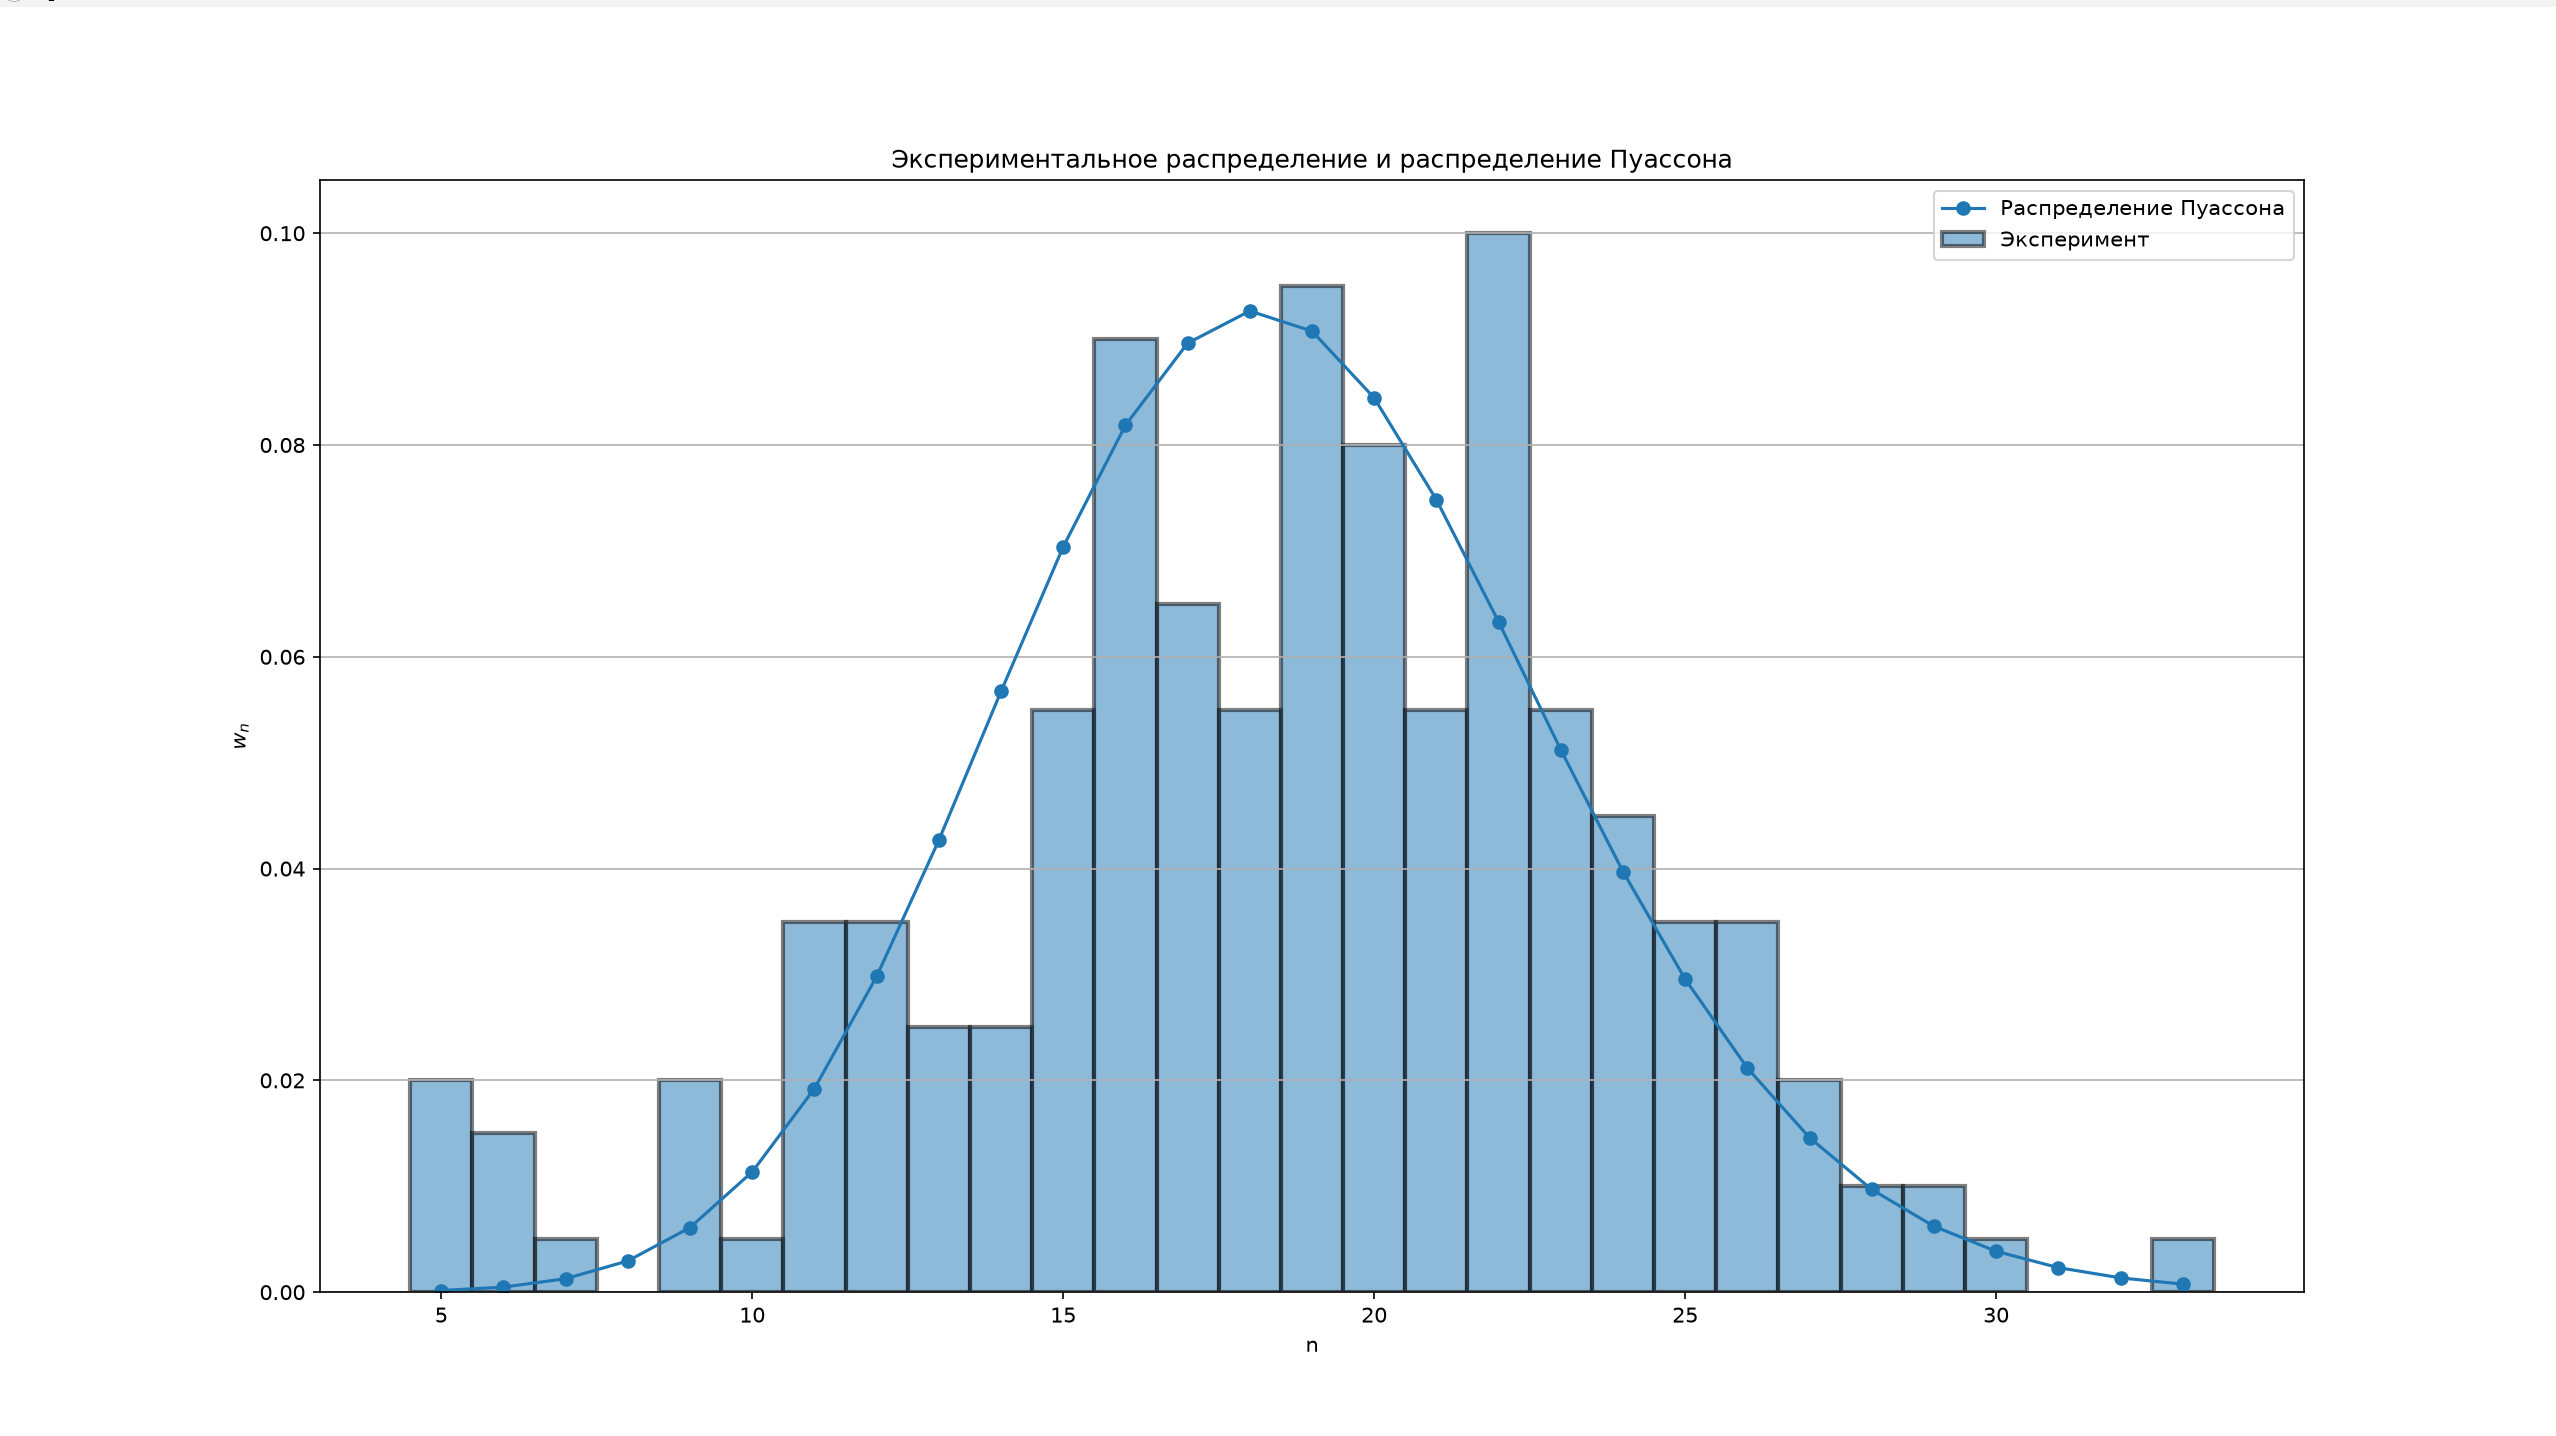
\includegraphics[width=0.85\textwidth]{+poisson.png}
    \caption{Экспериментальное распределение и распределение Пуассона при $\tau=20$~с}
    \label{fig:poisson}
\end{figure}

На рисунке~\ref{fig:gauss} экспериментальная гистограмма сопоставлена с нормальным распределением.

\begin{figure}[H]
    \centering
    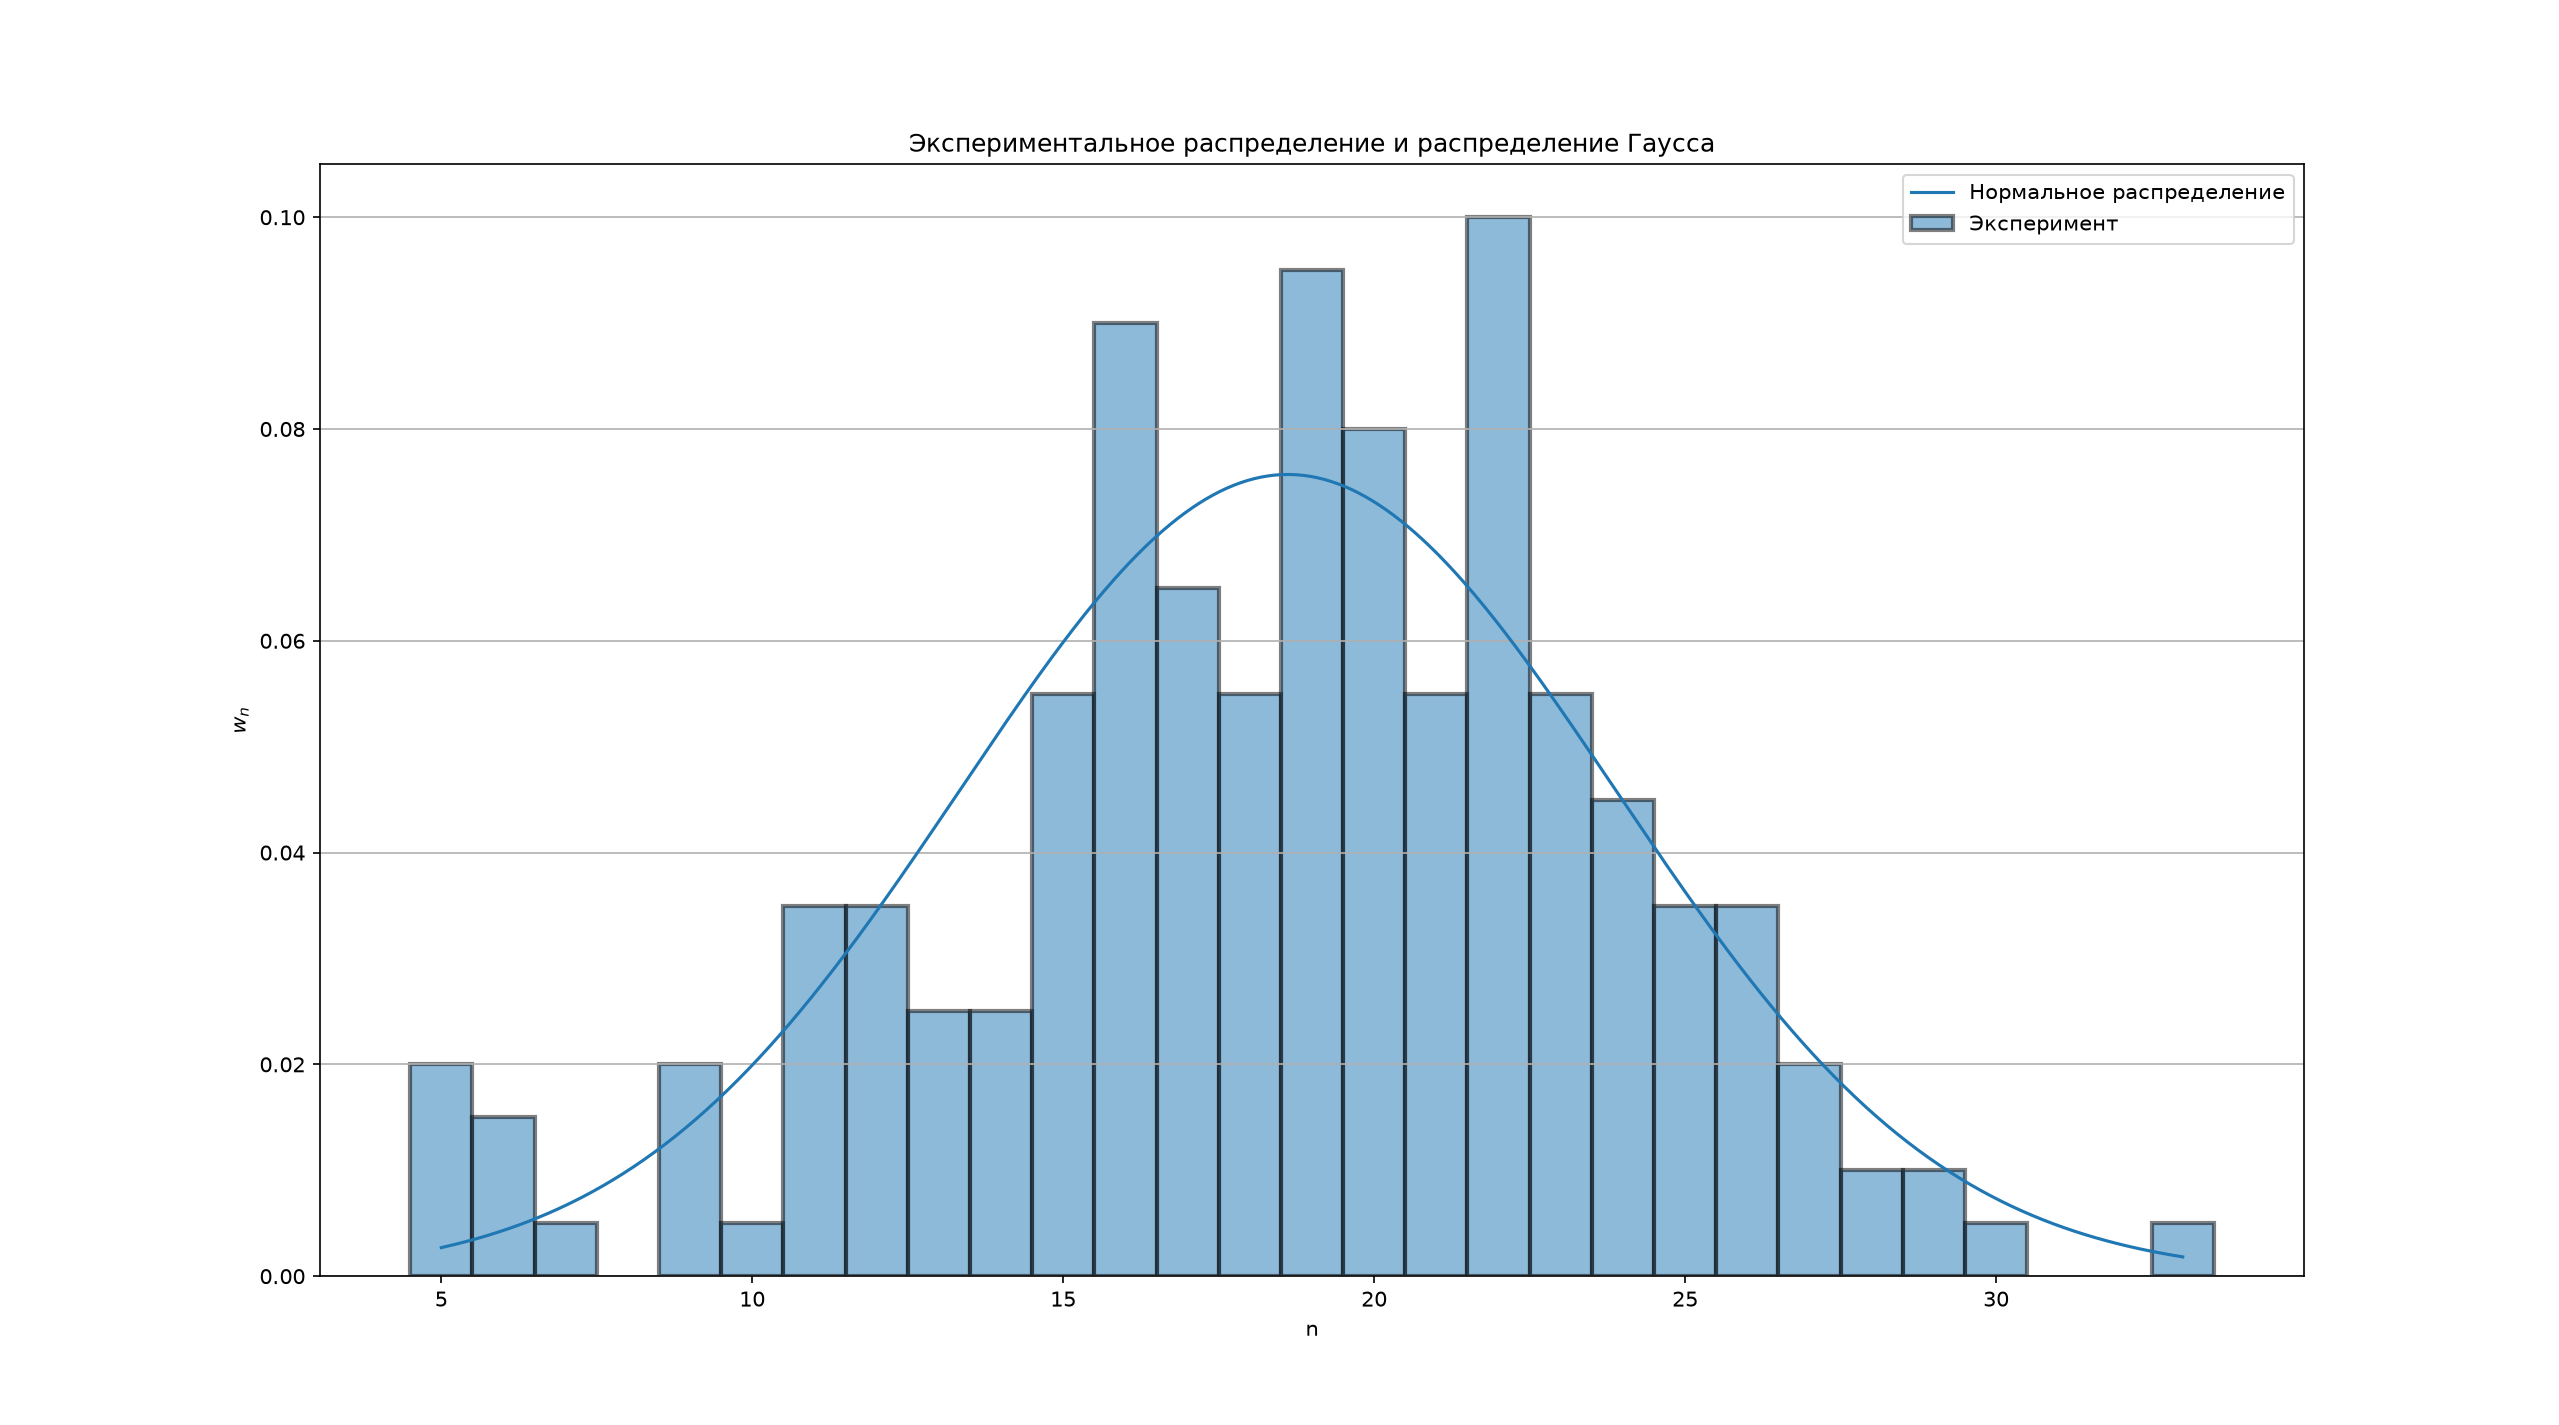
\includegraphics[width=0.85\textwidth]{+gauss.png}
    \caption{Экспериментальное распределение и нормальное распределение при $\tau=20$~с}
    \label{fig:gauss}
\end{figure}

Для непосредственного сравнения двух теоретических распределений с экспериментальными данными был также построен общий график, представленный на рисунке~\ref{fig:poisson_gauss}.

\begin{figure}[H]
    \centering
    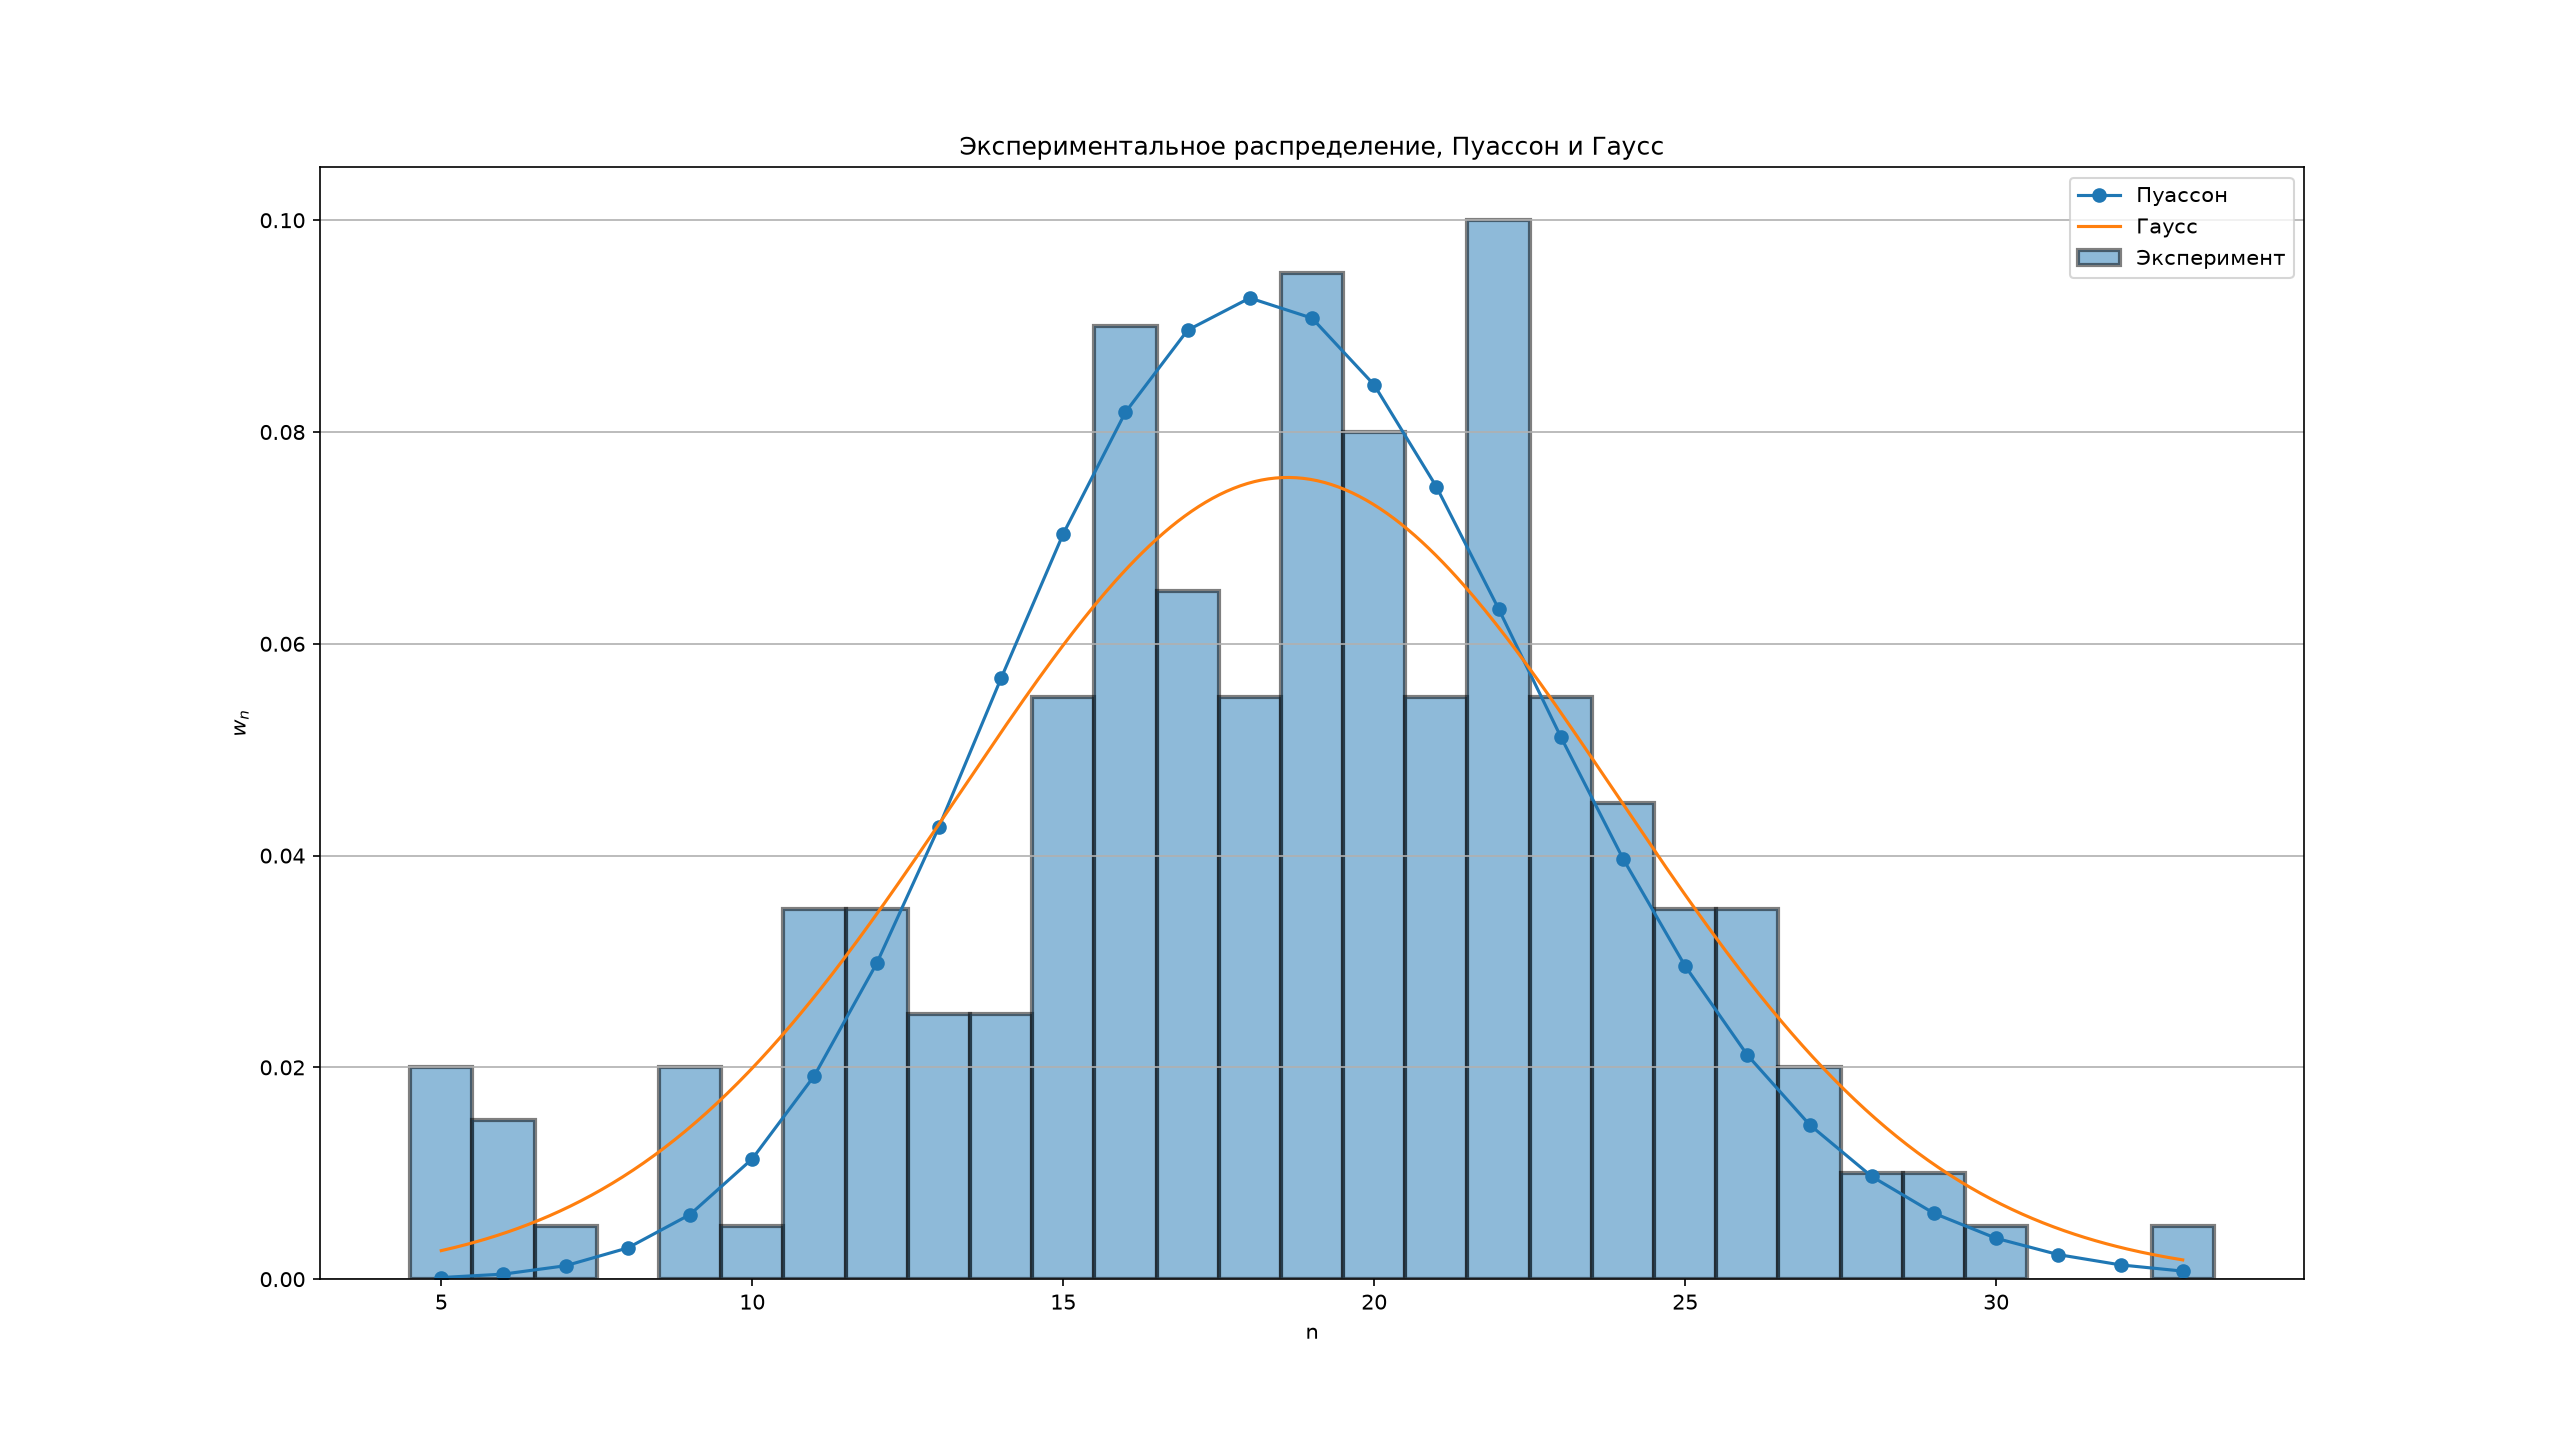
\includegraphics[width=0.85\textwidth]{+poisson+gauss.png}
    \caption{Сравнение экспериментального распределения с распределениями Пуассона и Гаусса}
    \label{fig:poisson_gauss}
\end{figure}

Из графиков видно, что оба теоретических распределения качественно описывают форму экспериментальной гистограммы. При этом распределение Пуассона непосредственно описывает дискретное число зарегистрированных частиц, тогда как нормальное распределение является его приближением при достаточно большом среднем значении $\langle n\rangle$.

\subsection*{2.5. Анализ погрешностей при различных разбиениях}

Для сравнения качества измерений при различных значениях $\tau$ рассмотрим относительную величину среднеквадратичного отклонения:

\begin{equation}
    \varepsilon_{\sigma}=
    \frac{\sigma_n}{\langle n\rangle}.
    \label{eq:relative_sigma}
\end{equation}

Получаем:

\[
\varepsilon_{\sigma,10}
=
\frac{3.582}{9.305}
\approx 0.385,
\]

\[
\varepsilon_{\sigma,20}
=
\frac{5.270}{18.61}
\approx 0.283,
\]

\[
\varepsilon_{\sigma,40}
=
\frac{7.886}{37.22}
\approx 0.212,
\]

\[
\varepsilon_{\sigma,80}
=
\frac{12.764}{74.44}
\approx 0.171.
\]

Таким образом, при увеличении времени группировки относительные флуктуации отдельного измерения уменьшаются:

\[
\varepsilon_{\sigma,10}
>
\varepsilon_{\sigma,20}
>
\varepsilon_{\sigma,40}
>
\varepsilon_{\sigma,80}.
\]

Это соответствует ожидаемому характеру статистических флуктуаций: чем больше частиц регистрируется за один интервал измерения, тем меньше относительный разброс числа зарегистрированных частиц.

Относительная погрешность среднего значения определяется как

\begin{equation}
    \varepsilon_{\langle n\rangle}
    =
    \frac{\sigma_{\langle n\rangle}}
    {\langle n\rangle}.
    \label{eq:relative_mean_error}
\end{equation}

Для полученных данных имеем:

\[
\varepsilon_{\langle n\rangle,10}
=
\frac{0.179}{9.305}
\approx 1.92\%,
\]

\[
\varepsilon_{\langle n\rangle,20}
=
\frac{0.373}{18.61}
\approx 2.00\%,
\]

\[
\varepsilon_{\langle n\rangle,40}
=
\frac{0.789}{37.22}
\approx 2.12\%,
\]

\[
\varepsilon_{\langle n\rangle,80}
=
\frac{1.805}{74.44}
\approx 2.42\%.
\]

Для строго пуассоновского процесса относительная погрешность среднего не зависела бы от $\tau$ и равнялась бы $\varepsilon_{\langle n\rangle}=1/\sqrt{n_\Sigma}$, где $n_\Sigma=\langle n\rangle N\approx3722$, то есть $\approx1.64\%$. В данном эксперименте значения больше и растут с увеличением $\tau$. Причина видна из соотношения
\[
\varepsilon_{\langle n\rangle}
=\frac{\sigma_n}{\langle n\rangle\sqrt{N}}
=\frac{\sigma_n}{\sqrt{\langle n\rangle}}\cdot\frac{1}{\sqrt{n_\Sigma}},
\]
в котором множитель $1/\sqrt{n_\Sigma}$ от $\tau$ не зависит, а отношение $\sigma_n/\sqrt{\langle n\rangle}$ растёт: оно равно $1.17$, $1.22$, $1.29$ и $1.48$ для $\tau=10$, $20$, $40$ и $80$~с соответственно. Уменьшение числа групп $N$ само по себе на $\varepsilon_{\langle n\rangle}$ не влияет, так как оно уже учтено в $n_\Sigma$.

Стандартные ошибки среднего при различных разбиениях составляют

\[
\sigma_{\langle n\rangle,10}=0.179,
\qquad
\sigma_{\langle n\rangle,20}=0.373,
\]

\[
\sigma_{\langle n\rangle,40}=0.789,
\qquad
\sigma_{\langle n\rangle,80}=1.805.
\]

Окончательные результаты определения среднего числа зарегистрированных частиц для каждого значения $\tau$ можно записать в виде

\[
\langle n\rangle_{10}=9.305\pm0.179,
\]

\[
\langle n\rangle_{20}=18.61\pm0.37,
\]

\[
\langle n\rangle_{40}=37.22\pm0.79,
\]

\[
\langle n\rangle_{80}=74.44\pm1.81.
\]

При этом во всех случаях получено одно и то же значение интенсивности регистрации:

\[
j=0.9305~\text{с}^{-1}.
\]

С учётом статистической погрешности интенсивность можно представить результатами

\[
j_{10}=(0.9305\pm0.0179)~\text{с}^{-1},
\]

\[
j_{20}=(0.9305\pm0.0186)~\text{с}^{-1},
\]

\[
j_{40}=(0.9305\pm0.0197)~\text{с}^{-1},
\]

\[
j_{80}=(0.9305\pm0.0226)~\text{с}^{-1}.
\]

Полученные результаты показывают, что изменение способа группировки исходных данных практически не влияет на определённую интенсивность космического излучения. При этом увеличение $\tau$ приводит к уменьшению относительных флуктуаций числа частиц в отдельном интервале, но одновременно уменьшает число независимых измерений.

\section*{3. Итоговый результат и выводы}

В качестве итогового результата принимаем значение, полученное при $\tau=10$~с, где погрешность наименьшая:

\[
j=(0.931\pm0.018)~\text{с}^{-1},
\qquad
\varepsilon_j\approx1.9\%.
\]

Результаты для остальных $\tau$ получены из тех же данных, поэтому независимыми не являются и отличаются только способом группировки. Погрешность определена по выборочному $\sigma_n$, так как оно отражает фактический разброс данных. Пуассоновская оценка $1/\sqrt{n_\Sigma}$ дала бы $1.6\%$.

\begin{itemize}
    \item Среднее число зарегистрированных частиц пропорционально $\tau$, а интенсивность $j=0.9305$~с$^{-1}$ не зависит от способа группировки.
    \item Экспериментальное $\sigma_n$ превышает $\sqrt{\langle n\rangle}$ на $17$--$48\%$, причём разность растёт с $\tau$. Следовательно, свойство $\sigma_n=\sqrt{\langle n\rangle}$ выполняется лишь приближённо. Относительная погрешность среднего растёт от $1.9\%$ до $2.4\%$ при ожидаемых $1.6\%$ для идеального пуассоновского процесса.
    \item Доли измерений в интервалах $\pm\sigma_n$, $\pm2\sigma_n$ и $\pm3\sigma_n$ ($67$--$68.5\%$, $93$--$95\%$ и $100\%$) согласуются с нормальным распределением, а форма гистограмм близка к гауссовой.
    \item Относительные флуктуации отдельного отсчёта убывают с ростом $\tau$ (от $0.385$ до $0.171$).
\end{itemize}

\end{document}